
\documentclass{article}
\usepackage[utf8]{inputenc}

\usepackage{amsmath,amsfonts,stmaryrd,amssymb} % Math packages

\usepackage{graphicx, float, subfigure} % Picture package

\usepackage{enumerate} % Custom item numbers for enumerations

\usepackage[ruled]{algorithm2e} % Algorithms

\usepackage[framemethod=tikz]{mdframed} % Allows defining custom boxed/framed environments

\usepackage{listings} % File listings, with syntax highlighting
\lstset{
	basicstyle=\ttfamily, % Typeset listings in monospace font
}

\usepackage{cite}
\usepackage{setspace}

%----------------------------------------------------------------------------------------
%	DOCUMENT MARGINS
%----------------------------------------------------------------------------------------

\usepackage{geometry} % Required for adjusting page dimensions and margins

\geometry{
	paper=a4paper, % Paper size, change to letterpaper for US letter size
	top=2.5cm, % Top margin
	bottom=3cm, % Bottom margin
	left=2.5cm, % Left margin
	right=2.5cm, % Right margin
	headheight=14pt, % Header height
	footskip=1.5cm, % Space from the bottom margin to the baseline of the footer
	headsep=1.2cm, % Space from the top margin to the baseline of the header
	%showframe, % Uncomment to show how the type block is set on the page
}

%----------------------------------------------------------------------------------------
%	FONTS
%----------------------------------------------------------------------------------------

\usepackage[utf8]{inputenc} % Required for inputting international characters
\usepackage[T1]{fontenc} % Output font encoding for international characters

\usepackage{XCharter} % Use the XCharter fonts

 % Include the file specifying the document structure and custom commands
\renewcommand{\baselinestretch}{1.2}

\setcounter{secnumdepth}{4}

\title{Comparison between Collaborative Filtering Algorithms: 
Weighted Bipartite Graph Projection and Alternating Least Squares} % Title of the assignment


\date{\today} 


\begin{document}

\maketitle % Print the title



\begin{center}
  {\Large Abstract}
\end{center}



\noindent This paper aims to compare the performance of two different collaborative 
filtering methods in aspect of prediction accuracy and time efficiency. The two approaches
chosen in this paper are the weighted bipartite graph projection (WBGP) approach with 
recommendation power as the similarity measure and the matrix factorization approach 
with alternating least squares (ALS) learning algorithm. The two algorithms are implemented 
on a small subset of Yelp Open Dataset where the businesses are all from Washington state and 
the root mean squared error (RMSE) is chosen as the evaluation metrics for the comparison. The 
implementation of the algorithms is based on Apache Spark platform in Python programming 
language (Pyspark). The result shows that although the alternating least squares (ALS) 
algorithm beats the weighted bipartite graph projection (WBGP) in terms of computational 
time, the latter can produce better prediction accuracy.


\section*{Introduction} % Unnumbered section

\noindent Recommender systems have become quite popular in recent years 
since e-commerce companies rose. They to a great extent help costumers discover what they 
need or are interested in and in the meantime improve the user experiences. At present, recommender 
systems have been applied almost anywhere, not only by e-commerce platforms like Amazon and Netflix 
but also by social platforms like Facebook and Instagram. Since the data for these companies are 
usually enormous, the systems are often required to be scalable to a huge amount of data and computations.

\indent Generally speaking, there are two main strategies in recommender systems: content 
filtering and collaborative filtering \cite{koren2009matrix}. The basic idea of content filtering is to construct 
a profile of a user or an item (products, businesses, movies etc.) with external information like 
the gender or salary of users and the genre or price of items. Content filtering believes that the 
information of these qualities can help capture the nature of users and items and therefore improve 
the prediction on users’ preferences. In contrast with it, collaborative filtering concentrates only 
on past user behaviors such as transactions and ratings. It studies the relationship between users and 
items to predict new user-item associations without any external information. 

\indent This paper focuses on comparison between two collaborative filtering approaches in two 
different areas: neighborhood methods and latent factor models \cite{koren2009matrix}. Neighborhood methods aim 
to find the similarities between users or items while latent factors models attempt to explain 
the transactions or ratings by some latent factors (the number of latent factors is usually far 
smaller than the number of all users or items). For neighborhood methods I apply the weighted bipartite 
graph projection (WBGP) approach proposed by \cite{zhou2007bipartite} with similarity measure defined in \cite{sawant2013collaborative} \cite{shang2008personal}; for latent factors 
model methods I employ the matrix factorization with alternating least squares (ALS) learning algorithm \cite{koren2009matrix}. 

\section*{Data} % Unnumbered section


\noindent The collaborative filtering approaches are implemented on Yelp Open Dataset

\noindent (https://www.yelp.com/dataset). Yelp.com is a crowd-sourced local business review and 
social networking site, and its open dataset mainly contains information of businesses, users 
and users’ reviews on businesses from 8 metropolitan areas in Canada and United States. Due to 
the limitation of cluster resources and run time, I only select businesses from Washington state 
and eliminate those have fewer than 15 reviews for reducing the sparseness of user-business matrix 
similar to \cite{ting2013yelp}. The summary of data this paper uses is shown in Table 1.

\begin{table}[H]
\centering
\begin{tabular}{|l|l|} 
\hline
Number of Businesses                   & 1589                \\ 
\hline
Number of Users                        & 44780               \\ 
\hline
Number of Reviews                      & 102383              \\ 
\hline
Average Number of Reviews for User     & 2.2863555158552926  \\ 
\hline
Average Number of Reviews for Business & 64.43234738829453   \\
\hline
\end{tabular}
\caption{Summary of Data}
\label{table1}
\end{table}



\section*{Methodology} % Unnumbered section

\subsection*{1  Weighted Bipartite Graph Projection}

\subsubsection*{1.1  Background and Concept}

\noindent Weight Bipartite Graph Projection (WBGP) approach is in the domain of 
neighborhood methods which focus on evaluating the similarities between users or items. 
These methods can be generally classified into two types: user-oriented and item-oriented. 
User-oriented methods learn similarities between users so they estimate unknown ratings based 
on recorded ratings of like-minded users; item-oriented methods learn similarities between items 
so they make predictions based on recorded ratings made by the same user on similar items. WBGP 
approach can be implemented from both perspectives. This paper applies the item-oriented 
(business-oriented) WBGP method on account of its better scalability and improved accuracy 
in many cases \cite{hu2008collaborative}. Note that user-oriented method is mathematically equivalent by just switching 
the roles of item and user.


\indent A bipartite graph is a graph where the set of vertices are partitioned 
in two disjoint sets X and Y such that each edge of the graph connects two vertices only 
in different sets (as illustrated in Figure 1(a)). The projection of bipartite graph onto one set, 
for example X, is a graph whose nodes only come from the set X and they are connected with each other 
when they have at least one common neighboring Y node in the original bipartite graph. 
If we additionally assign some “weights” to each edge in the projection, we then get the weighted 
bipartite graph projection (as illustrated in Figure 1(b) and Figure 1(c)). The simplest weight 
assigned to each edge is the number of common neighboring Y nodes the two vertices have which is 
exactly the case in Figure 1. Beyond that we can also assign similarity measures which are more 
complicated in order to capture the relationship between each pair of nodes from the original graph. 
There are some popular similarity functions usually applied in neighborhood approaches such as Pearson 
correlation similarity, Cosine similarity and Tanimoto coefficient \cite{kupisz2015collaborative}. The similarity measure applied 
in this paper is defined in \cite{sawant2013collaborative} \cite{shang2008personal}as a measure of recommendation power.

% Picture insertion
\begin{figure}[H]
	\centering
	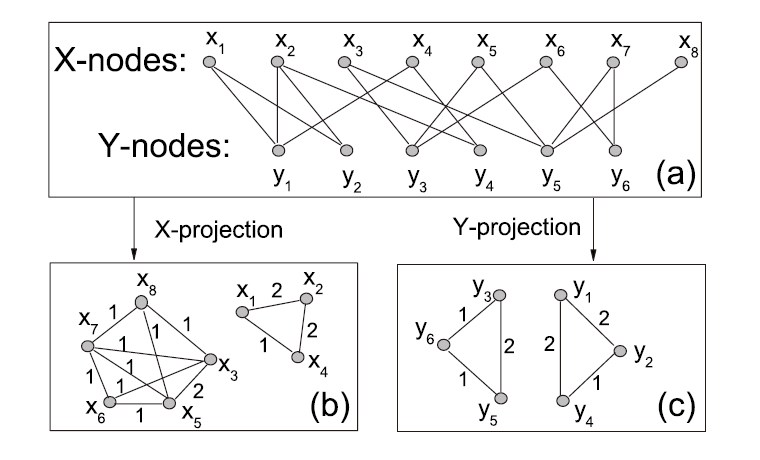
\includegraphics[width = .8\textwidth]{figs/figure1.png}
	\caption{Diagram of Weighted Bipartite Graph Projection} 
	\label{figure1}
\end{figure}





\subsubsection*{1.2  Similarity Measure}


\noindent As mentioned above, similarity measures can be thought of as the weights assigned 
to each edge in a WBGP. However, the WBGP we talked about in the previous section is undirected, 
meaning the similarity or weight between two nodes is the same. This situation is suitable for 
symmetric similarity measures like Pearson correlation similarity and Cosine similarity because 
if we switch the role of the two nodes the similarity remains unchanged. Now we consider a directed 
WBGP that doubles the edges of the undirected one since there are two edges between each pair of 
nodes. With this directed graph projection, we need to apply an asymmetric similarity measure 
(i.e. $sim(i, j) = sim(j, i)$ does not always hold) for each edge. The recommendation power measure 
can capture the asymmetric features in any pairs of businesses $i, j$ and is defined as

% Math equation/formula
\begin{equation}
	rp\left ( i,j \right )=\sum_{u\in U}^{}\frac{r_{i,u}r_{j,u}}{R_{i}R_{u}}
\end{equation}


\noindent where $U$ is the set of all users who have rated both $i$ and $j$, $r_{i,u}$ is the rating that 
user $u$ gives to business $i$, $R_{i}$ is the sum of ratings business $i$ has received and $R_{u}$ is the sum of 
ratings user $u$ has given. 


\indent This measure is obviously asymmetric due to the existence of $R_{i}$. Actually, 
the recommendation power measure represents how likely business $j$ is to appeal to a particular 
user provided that he or she has been to business $i$ and rated it according to \cite{sawant2013collaborative}, hence it gives a 
reasonable explanation for why this measure is asymmetric.

\subsubsection*{1.3  Algorithm}


\noindent First I build a bipartite graph (one set for users and the other for businesses) with 
weights as ratings using the Yelp review data. Next I calculate the recommendation power for all 
pairs of businesses according to equation (1) and build the weighted bipartite graph projection on 
the business set. Finally, the prediction of rating from user $u$ to business $i$ can be computed by the 
following formula which is similar to the one in \cite{sawant2013collaborative} \cite{breese2013empirical}(simply transfer from user-oriented aspect to 
business-oriented aspect):

% Math equation/formula
\begin{equation}
	\hat{r}_{i,u} = \bar{r_{i}}+\sum_{j\in B_{u}}^{}rp\left ( i,j \right )\left ( r_{j,u}-\bar{r_{j}} \right ).
\end{equation}

\noindent Here $\bar{r_{i}}$ represents the average rating received by business $i$ and $B_{u}$ is the set of 
businesses the user $u$ has ever rated. Notice that in the extremely sparse situation where the 
recommendation power measures from business $i$ to any other businesses are all 0, the predicted 
rating of business $i$ given by any new user $u$ simply equals to the average rating of business $i$. 


\subsection*{2  Matrix Factorization with Alternating Least Squares}

\subsubsection*{2.1  Background and Concept}


\noindent Matrix factorization is one of the widely successful latent factor models which 
characterizes both items and users by vectors of factors inferred from item rating patterns. 
Imagine a user-item matrix $M_{m\times n}$ with some known entries representing the feedback or preference 
a user giving to an item, for instance ratings, the task of collaborative filtering is to fill in 
the missing entries of the matrix with predictions. Matrix factorization solves this problem by mapping 
both users and items to a joint latent factor space of dimensionality $k$ (usually much smaller than the 
number of users or items), such that user-item interactions are modeled as inner products in that space 
\cite{koren2009matrix}. We can express the idea mathematically as

% Math equation/formula
\begin{equation}
	\hat{M_{i,j}}=u_{i}^{T}v_{j} \qquad where\ \ u_{i}\in R^{k}\ and\ v_{j}\in R^{k}
\end{equation}



\noindent where $\hat{M_{i,j}}$ is the predicted rating given by user $i$ to item $j$, $u_{i}$ is a parameter 
vector associated with user $i$ and $v_{j}$ is a parameter vector associated with item $j$. More generally, 
we can get the matrix expression:

% Math equation/formula
\begin{equation}
	\hat{M} = U^{T}V \qquad where\ U=\left [ u_{1},...,u_{n} \right ]\ and\ V=\left [ v_{1},...,v_{m} \right ].
\end{equation}

\noindent Here $n$ and $m$ are the numbers of users and items respectively, and $\bar{M}$ represents the 
whole predicted user-item matrix.

\indent To achieve the parameter vectors for each user and item, we consider minimize the 
following loss function:

% Math equation/formula
\begin{equation}
	f\left ( U,V \right )=\sum_{\left ( i,j \right )\in \Omega }^{}\left ( M_{i,j} - u_{i}^{T}v_{j}\right )^{2}+\lambda \left ( \sum_{i=1}^{n}\left \| u_{i} \right \|^{2}+\sum_{j=1}^{m}\left \| v_{j} \right \|^{2} \right ).
\end{equation}

\noindent Here $\Omega$ is the set of $\left ( i,j \right )$ pairs for which $M_{i,j}$ is known and $\lambda \geq 0$ is a 
regularization hyper-parameter. This loss function can be derived using the Bayesian model \cite{st446lecturenotes}.

\subsubsection*{2.2  Learning Algorithm}


\noindent Minimizing the loss function above is a non-convex optimization problem, so traditional 
gradient descent algorithm can only converge to local minima and might also be very slow. Therefore, 
this paper applies alternating least squares (ALS) algorithm which performs better in many cases.



\indent The main idea of ALS is to fix one of the unknowns $u_{i}$ and $v_{j}$ in the loss function 
and optimize the other by solving a least squares problem. The algorithm rotates between fixing 
$u_{i}$’s and fixing $v_{j}$’s utill some termination criteria are met. Since each phase corresponds to solving a 
convex optimization problem, it ensures that each phase decreases the loss function until convergence \cite{koren2009matrix}.

\subsubsection*{2.3  Hyperparameters Selection}

\noindent In matrix factorization with ALS algorithm we have three hyperparameters to choose: 
the number of latent factors $K$, the max number of iterations $I$ (termination criterion) and the 
regularization parameter $\lambda$. First I set a fixed grid for $K$ and $I$, and try different values for 
$\lambda$ (0.1, 0.5 and 1). The models are trained on the training data and the root mean squared errors 
(RMSE) are computed using the test data. The results for different $\lambda$ values are shown respectively 
in Figure 2, Figure 3 and Figure 4. The figures indicate that the models with $\lambda$ equaling to 0.5 and $K$ 
equaling to 3 perform better in general. The result also shows that RMSE decreases as $I$ increases, 
hence I move the grid of $I$ forward to see if more iterations can result in better accuracy. However, 
Figure 5 (in Appendix) displays that the RMSE decreases very slowly after 10 iterations, meaning the 
algorithm gets extremely close to the optimum value so it makes little sense to infinitely increase I. 
Finally, I select the model with $K=3$, $I=14$ and $\lambda =0.5$ as the best one.


% Picture insertion
\begin{figure}[H]
	\centering
	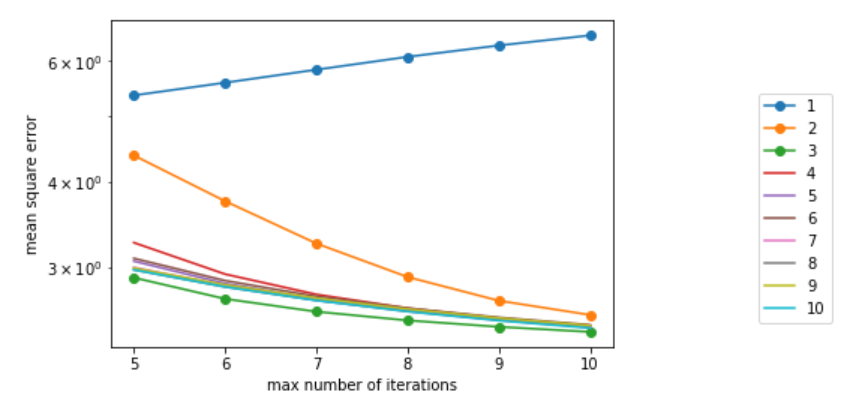
\includegraphics[scale=0.5]{figs/figure2.png}
	\caption{Test RMSE for Models with $\lambda =0.1$} 
	\label{figure2}
\end{figure}


% Picture insertion
\begin{figure}[H]
	\centering
	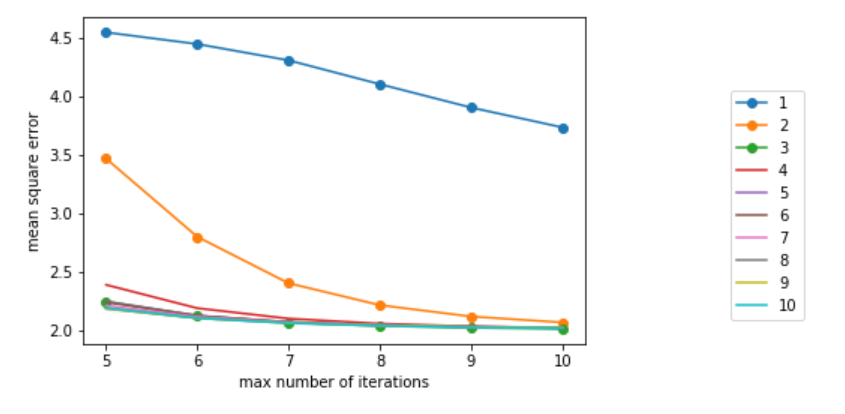
\includegraphics[scale=0.5]{figs/figure3.png}
	\caption{Test RMSE for Models with $\lambda =0.5$} 
	\label{figure3}
\end{figure}


% Picture insertion
\begin{figure}[H]
	\centering
	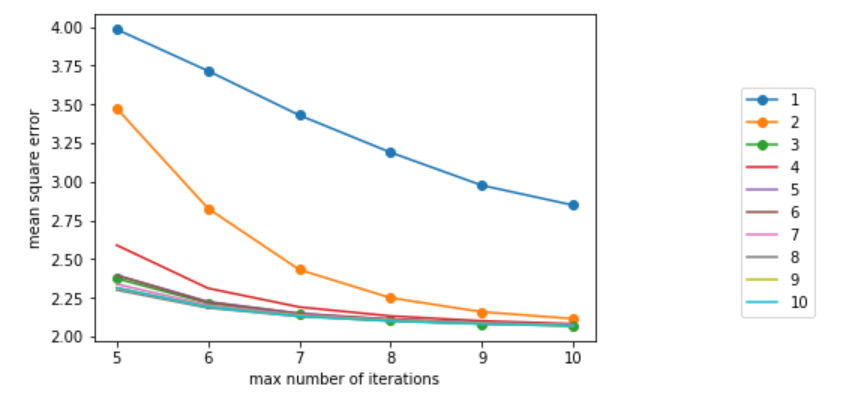
\includegraphics[scale=0.5]{figs/figure4.png}
	\caption{Test RMSE for Models with $\lambda =1$} 
	\label{figure4}
\end{figure}

\section*{Apache Spark} % Unnumbered section


\noindent In collaborative filtering based on neighborhood approaches, it is often quite expensive 
to calculate the similarities between users or items because the algorithms always need to search the 
entire dataset to find the neighbor of a particular user or item. According to \cite{kupisz2015collaborative}, the time complexity 
in the worst case can achieve $O(UI)$ ($U$ and $I$ are numbers of users and items respectively). In order to 
deal with the scalability problem, I choose Apache Spark which is a unified analytics engine for big 
data processing to implement the collaborative filtering algorithms in this paper. It can parallelize 
the algorithms using distributed systems and thus largely improve the computational efficiency. Moreover, 
the work of Kupisz and Unold \cite{kupisz2015collaborative} also proved that the system based on Apache Spark is more efficient than 
Hadoop with respect to the item-based collaborative filtering algorithm. In this paper, the collaborative 
filtering algorithms for the Apache Spark platform are implemented in the Python programming 
language (Pyspark).

\indent For implementation of the WBGP algorithm I mainly use the Dataframe APIs and some APIs 
in the GrahpFrame package like aggregateMessages and for implementation of the ALS algorithm I directly 
employ APIs in the pyspark.ml package like ALS.


\section*{Result} % Unnumbered section

\noindent To compare the prediction accuracy of the two algorithms, I randomly split the Yelp data into 
two sets: one for training (80\%) and one for test (20\%). The two algorithms are trained on the training 
set and the RMSE is calculated with respect to the test set. The whole process is repeated for 5 times 
and we get the mean and standard error of RMSE for both algorithms. The summarized result is shown in Table 2.

\indent Surprisingly, the WBGP approach performs not only better but also more stable than the ALS 
method. Besides, the mean of RMSE for the WBGP approach is quite similar to the result in \cite{sawant2013collaborative}.

\begin{table}[H]
\centering
\begin{tabular}{|l|l|l|} 
\hline
                       & WBGP                  & ALS                   \\ 
\hline
Mean of RMSE           & 1.4032339302172345    & 2.256193268649647     \\ 
\hline
Standard Error of RMSE & 0.0048709873291408355 & 0.018367415714108097  \\
\hline
\end{tabular}
\caption{Summarized Result of RMSE}
\label{table2}
\end{table}


\section*{Conclusion} % Unnumbered section

\noindent As two completely different collaborative filtering approaches, the WBGP and ALS algorithms 
have their own advantages and disadvantages. In terms of prediction accuracy, the WBGP method outperforms 
the ALS method with its average RMSE equaling to about 1.4. In addition, the standard error of RMSE with 
respect to WBGP is also smaller than ALS, indicating its superior stability. However, in terms of 
computational time, the ALS algorithm has great advantage over the WBGP algorithm since it has smaller 
time complexity \cite{st446lecturenotes} than WBGP. Actually, when I implement the two algorithms on Pyspark, the WBGP algorithm 
takes more than 10 times as long as the ALS algorithm takes.

\section*{Reflection and Further Research} % Unnumbered section

\noindent On account of the large time complexity of the WBGP algorithm and the limitation of cluster 
resources, the two approaches in this paper are only implemented on a small subset of the entire Yelp 
review dataset, which cannot make full use of the advantages brought by distributed computing. Larger 
datasets could be tried in further research.

\indent In collaborative filtering tasks we assume that one user can only have one rating on a particular 
item or business. However, it is usually not the case in the real-world data since users absolutely have 
rights to express his or her preference for an item several times. This problem also appears in the 
Yelp review dataset and what I do is dropping the redundant ratings for each user-item pair randomly. 
I think maybe better ways are to calculate the mean value of the ratings and regard it as the overall 
preference of the user to that item, or take the rating the user gave to that item most recently as 
the latest feedback. Perhaps in future papers these methods can be taken into consideration.

\indent In the implementation of the WBGP algorithm, ideally the recommendation power should be 
calculated directly from the bipartite graph by some graph algorithms like random walk in \cite{sawant2013collaborative}, but 
unfortunately I could not find any related APIs in the GraphFrames package in Pyspark so I calculate 
the recommendation power using some Dataframe APIs on the original data instead. However, I notice that 
Neo4j which is a graph database platform has an implementation of the random walk algorithm \cite{needham2019graph}. Further 
research could try implement the WBGP algorithm using Neo4j and see if it is more efficient than Apache Spark.

\clearpage

\bibliographystyle{plain}   
\bibliography{references}  % Reference



\section*{Appendix} % Unnumbered section

% Picture insertion
\begin{figure}[H]
	\centering
	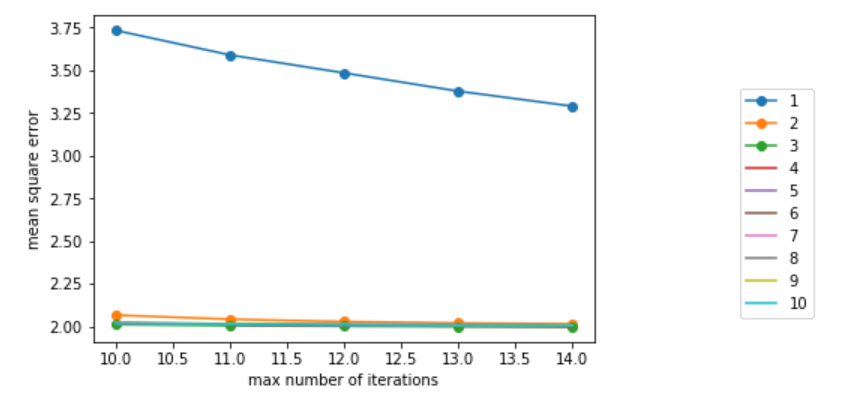
\includegraphics[width = .8\textwidth]{figs/figure5.png}
	\caption{Test RMSE for Models with $I=10,11,12,13,14$ and  $\lambda =0.5$} 
	\label{figure5}
\end{figure}



\end{document}
